\documentclass[11pt,aspectratio=169,reqno]{beamer}

\usepackage[labelformat=empty]{caption}
\usepackage[version=4]{mhchem}
\usepackage{multirow}
\usepackage{tabularx}
\usepackage{listings}

\usepackage{tikz}
\usetikzlibrary{arrows.meta}

\usepackage{biblatex}
\addbibresource{../sources.bib}

\title{Einfache Differentialgleichungssysteme zur Autoregulation}%Einfache Differentialgleichungssysteme zur Autoregulation ?
\date[28.03.2023]{28.03.2023}
\author{Mario Kunz, Xaver Hanushevsky}
\institute{D-BIOL}

\usetheme{eth}

\colorlet{titlefgcolor}{ETHBlue}
\colorlet{accentcolor}{ETHRed}

\newcommand{\highlightpause}{\addtocounter{beamerpauses}{-1}\pause\color<+>{ETHPurple}}

\begin{document}

\setlength{\titleboxwidth}{0.65\textwidth}
\titleframe

% Wer die bessere Idee hat
\begin{frame}[fragile]{Ist das relevant für mich?}
    \begin{figure}
        \centering
        \includegraphics[width=.8\textwidth]{images/WhatEvenIsThis.png}
    \end{figure}
    \pause
    \begin{tikzpicture}[remember picture,overlay]
       \node at (current page.center) {\includegraphics[width=0.8\paperwidth]{images/SystembiologieVVZ.png}};
    \end{tikzpicture}
\end{frame}

\begin{frame}{Ziel unserer Arbeit}
\begin{columns}
    \column{.5\textwidth}

    \begin{itemize}
        \item Mathematisches Modell für
        \begin{enumerate}
            \item negative Autoregulation
            \item positive Autoregulation
        \end{enumerate}
        \item mRNA- und Protein-Konzentration soll beachtet werden
        \begin{itemize}
            \item Verhältnis mRNA:Protein untersuchbar
        \end{itemize}
        \item numerische Lösung mit MATLAB
        \begin{itemize}
            \item \emph{da die Systeme nicht analytisch lösbar sein werden}
        \end{itemize}
    \end{itemize}
    
    \column{.5\textwidth}
    \begin{figure}
        \centering
        \includegraphics[width=.7\textwidth]{images/repression.png}
        \caption{\tiny Negative Autoregulation}
    \end{figure}
\end{columns}
\end{frame}

% Xaver
\begin{frame}{Rückkopplung im Kontext der Genexpression}
\begin{columns}
    \column{.5\textwidth}
    \centering
    \textbf{Positive Rückkopplung}
    \begin{figure}
        \includegraphics[width=.6\textwidth]{images/dna_positive_autoregulation.png}
    \end{figure}

    Gebundenes Protein führt zu Rekrutierung von RNA Polymerase\\[1em]
    mehr Protein $\Rightarrow$ \textbf{mehr} Protein
    \vspace{1em}

    \uncover<2->{
        \begin{tabular}{l | l}
            initiale Konzentration = 0 & nie Protein \\
            \hline
            Verhalten gegen $t=\infty$ & intuitiv $[\text{P}]=\infty$
        \end{tabular}
    }
    \only<3>{
        \begin{tikzpicture}[remember picture,overlay]
            \node[xshift=0.8cm, yshift=-4cm] at (current page.center) {\textcolor{ETHRed}{macht das Sinn?}};
            \draw[ETHRed, line width=1pt, arrows = {-Stealth[length=8pt, inset=2pt]}] (0,-0.8) -- (-0.7,-0.4);
        \end{tikzpicture}
    }
    
    \column{.5\textwidth}
    \centering
    \textbf{Negative Rückkopplung}
    \begin{figure}
        \includegraphics[width=.6\textwidth]{images/dna_negative_autoregulation.png}
    \end{figure}
    Freier Operator erlaubt Transkription\\[2em]
    mehr Protein $\Rightarrow$ \textbf{weniger} Protein
    \vspace{1em}

    \uncover<4->{
        \begin{tabular}{ l | l }
            initiale Konzentration = 0 & sofortige Ausprägung \\
            \hline
            Verhalten gegen $t=\infty$ & ?
        \end{tabular}
    }
    
\end{columns}
\end{frame}

% Mario
\begin{frame}{Negative Autoregulation über mRNA und Repressorprotein}
    \centering Nur freie DNA führt zu Transkription\\[1em]
    mehr Protein $\Rightarrow$ \textbf{weniger} freie DNA $\Rightarrow$ \textbf{weniger} Transkription $\Rightarrow$ \textbf{weniger} Protein

    \vspace{2em}

    \begin{figure}
        \centering
        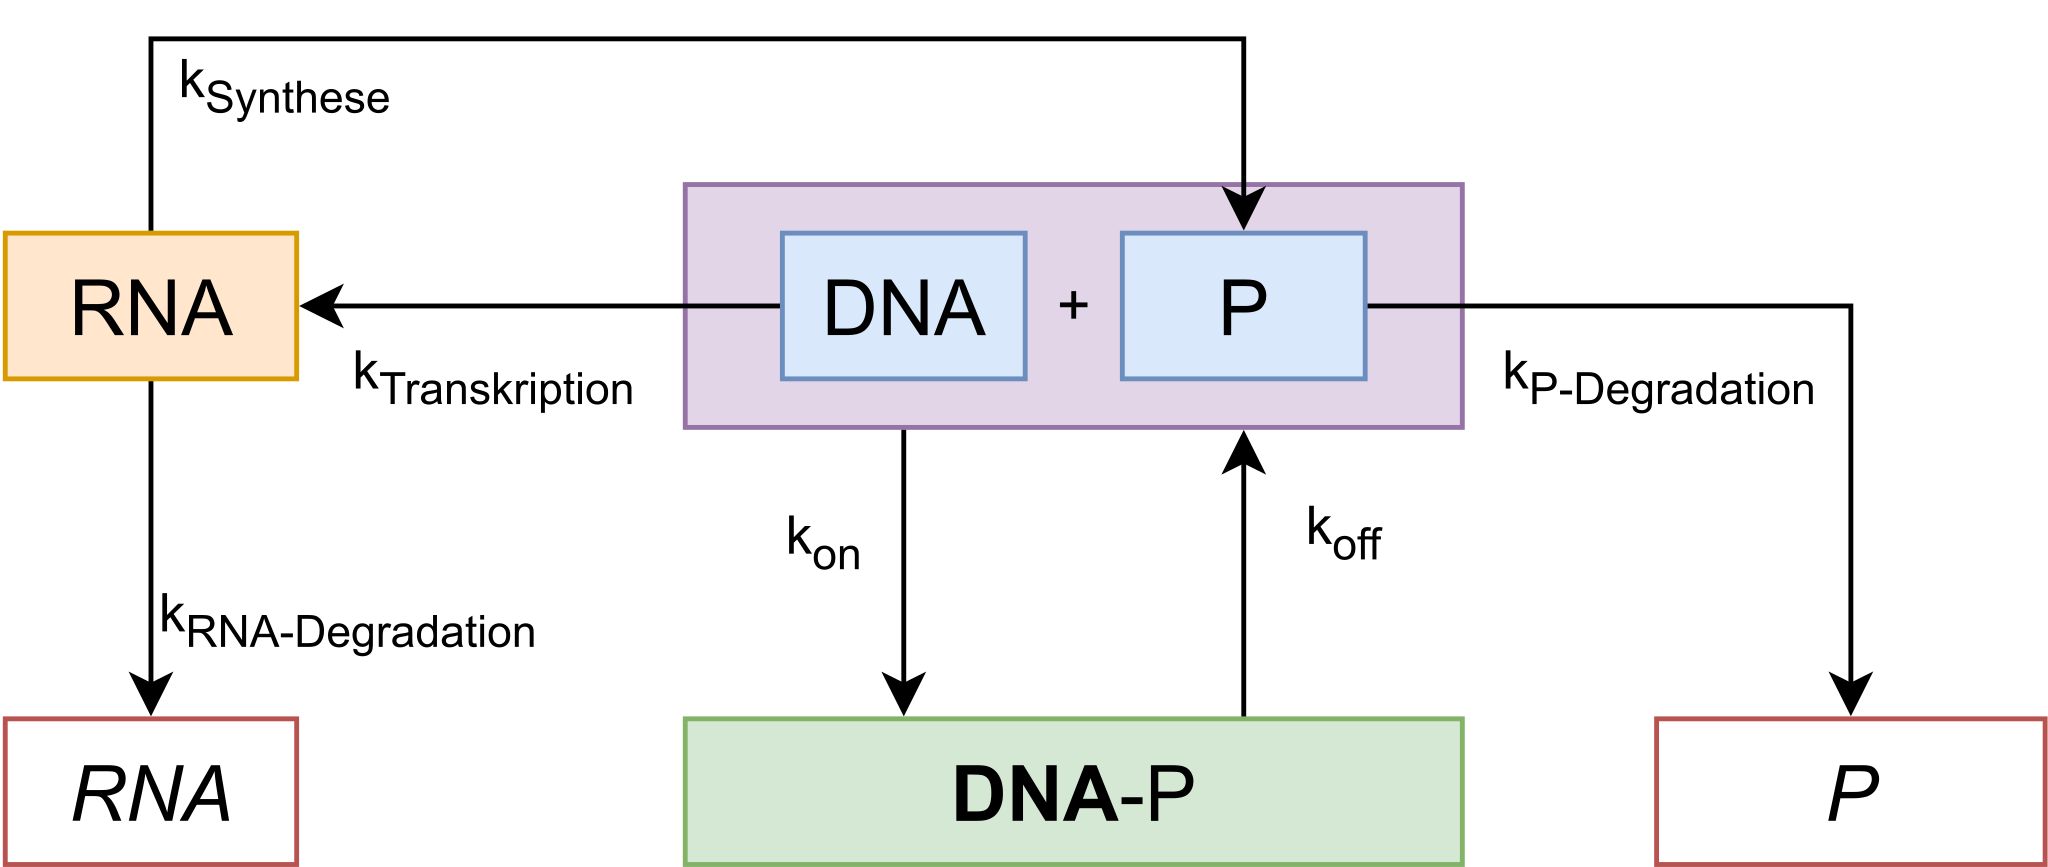
\includegraphics[width=.6\textwidth]{images/negative_autoregulation_overview.png}
    \end{figure}
\end{frame}

% Mario
\begin{frame}{Gleichgewicht zwischen gebundener und freier DNA}
    \begin{tikzpicture}[remember picture,overlay]
        \node[xshift=-2cm,yshift=-1.5cm] at (current page.north east) {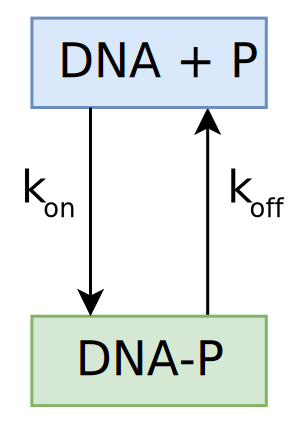
\includegraphics[width=2cm]{images/DNA-binding_equilibrium.png}};
    \end{tikzpicture}

    Hin- und Rückreaktionen im Gleichgewicht
    \begin{itemize}
        \item $v_\text{on}=k_\text{on}\cdot [\text{DNA}]\cdot [\text{P}]$
        \item $v_\text{off}=k_\text{off}\cdot [\text{DNA-P}]$\pause
    \end{itemize}

    \vspace{1.5em}

    \begin{columns}[onlytextwidth]
    \column{.4\textwidth}
    Für die folgenden Schritte nehmen wir an, dass sich das DNA-Protein Gleichgewicht sehr schnell einstellt, denn dann gilt:
    \column{.6\textwidth}
    \begin{itemize}
        \item $v_\text{on}=v_\text{off}$\\[8pt]
        \item $\dfrac{d[\text{DNA}]}{dt}=\dfrac{d[\text{DNA-P}]}{dt}=0$\\[8pt]
    \end{itemize}
    \[k_\text{on}\cdot [\text{DNA}]\cdot [\text{P}]=k_\text{off}\cdot [\text{DNA-P}]\]
    \end{columns}
\end{frame}

% Mario
\begin{frame}{Gleichgewicht zwischen gebundener und freier DNA}
    \begin{columns}[T]
    \column{.3\textwidth}
    \centering
    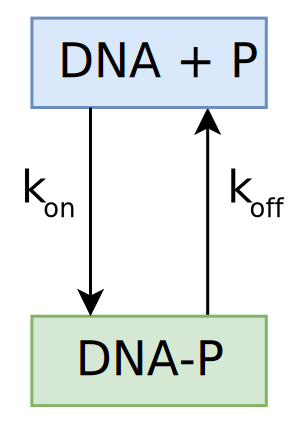
\includegraphics[width=2cm]{images/DNA-binding_equilibrium.png}
    \column{.3\textwidth}
    \[K_d=\frac{k_\text{off}}{k_\text{on}}=\frac{[\text{DNA}]\cdot [\text{P}]}{[\text{DNA-P}]}\]\pause
    \column{.3\textwidth}
        \[[\text{DNA$_\text{Total}$}]=[\text{DNA}]+[\text{DNA-P}]\]\\[-2em]
        \[[\text{DNA}]=[\text{DNA$_\text{Total}$}]-[\text{DNA-P}]\]
    \end{columns}

    \vspace{4em}
    \highlightpause
    
    \parbox{\textwidth}{
    % \[\Downarrow\]
    % \[K=\frac{([\text{DNA$_\text{Total}$}]-[\text{DNA-P}])\cdot [\text{P}]}{[\text{DNA-P}]}\]\\
    % \[K\cdot[\text{DNA-P}]=[\text{DNA$_\text{Total}$}]\cdot [\text{P}]-[\text{DNA-P}]\cdot [\text{P}]\]
    % \[[\text{DNA-P}]\cdot(K+[\text{P}])=[\text{DNA$_\text{Total}$}]\cdot [\text{P}]\]\\
    \[[\text{DNA-P}]=\frac{[\text{DNA$_\text{Total}$}]\cdot [\text{P}]}{K+[\text{P}]}\]
    }
\end{frame}

% Mario
\begin{frame}{Vergleich mit Bindungsgleichgewichte, Grundlagen der Biologie 1}
    \begin{columns}
        \column{.4\textwidth}
        Konzentration der besetzten DNA\vspace{1em}
        \[[\text{DNA-P}]=[\text{DNA$_\text{Total}$}]\cdot\color{ETHPurple}\frac{[\text{P}]}{K_d+[\text{P}]}\]
        \pause
        
        \column{.6\textwidth}
        \begin{figure}
            \centering
            \includegraphics[width=.6\textwidth]{images/occuption_degree_glockshuber.png}
            \caption*{\tiny Skript Prof. Dr. Rudolf Glockshuber, S. 32}
        \end{figure}
        
        \begin{description}
            \item[$K_\text{Diss}$] Dissoziationskonstante der Protein-Ligand-Paares
            \item[$\lbrack L_\text{tot}\rbrack$] Totale Konzentration des Liganden
            \item[$y$] Besetzungsgrad des Proteins
            \item[$K_\text{Diss}=\lbrack L_\text{tot}\rbrack$] 50\% des Proteins sind besetzt
        \end{description}
    \end{columns}
\end{frame}


% Mario
\begin{frame}{Vom Besetzungsgrad zum Nichtbesetzungsgrad}
\begin{block}{Negative Autoregulation}
    RNA wird \textbf{nur} transkribiert, wenn die DNA \textbf{nicht} besetzt ist
\end{block}

\begin{align*}
    z&=1-\frac{[\text{P}]}{K_d+[\text{P}]}\\[2em]
    z&=\frac{K_d}{K_d+[\text{P}]}\\[2em]
    [\text{DNA}]&=[\text{DNA}_\text{Total}]\cdot \frac{K_d}{K_d+[\text{P}]}
\end{align*}


\end{frame}

% Xaver
\begin{frame}{Mathematische Modellierung}

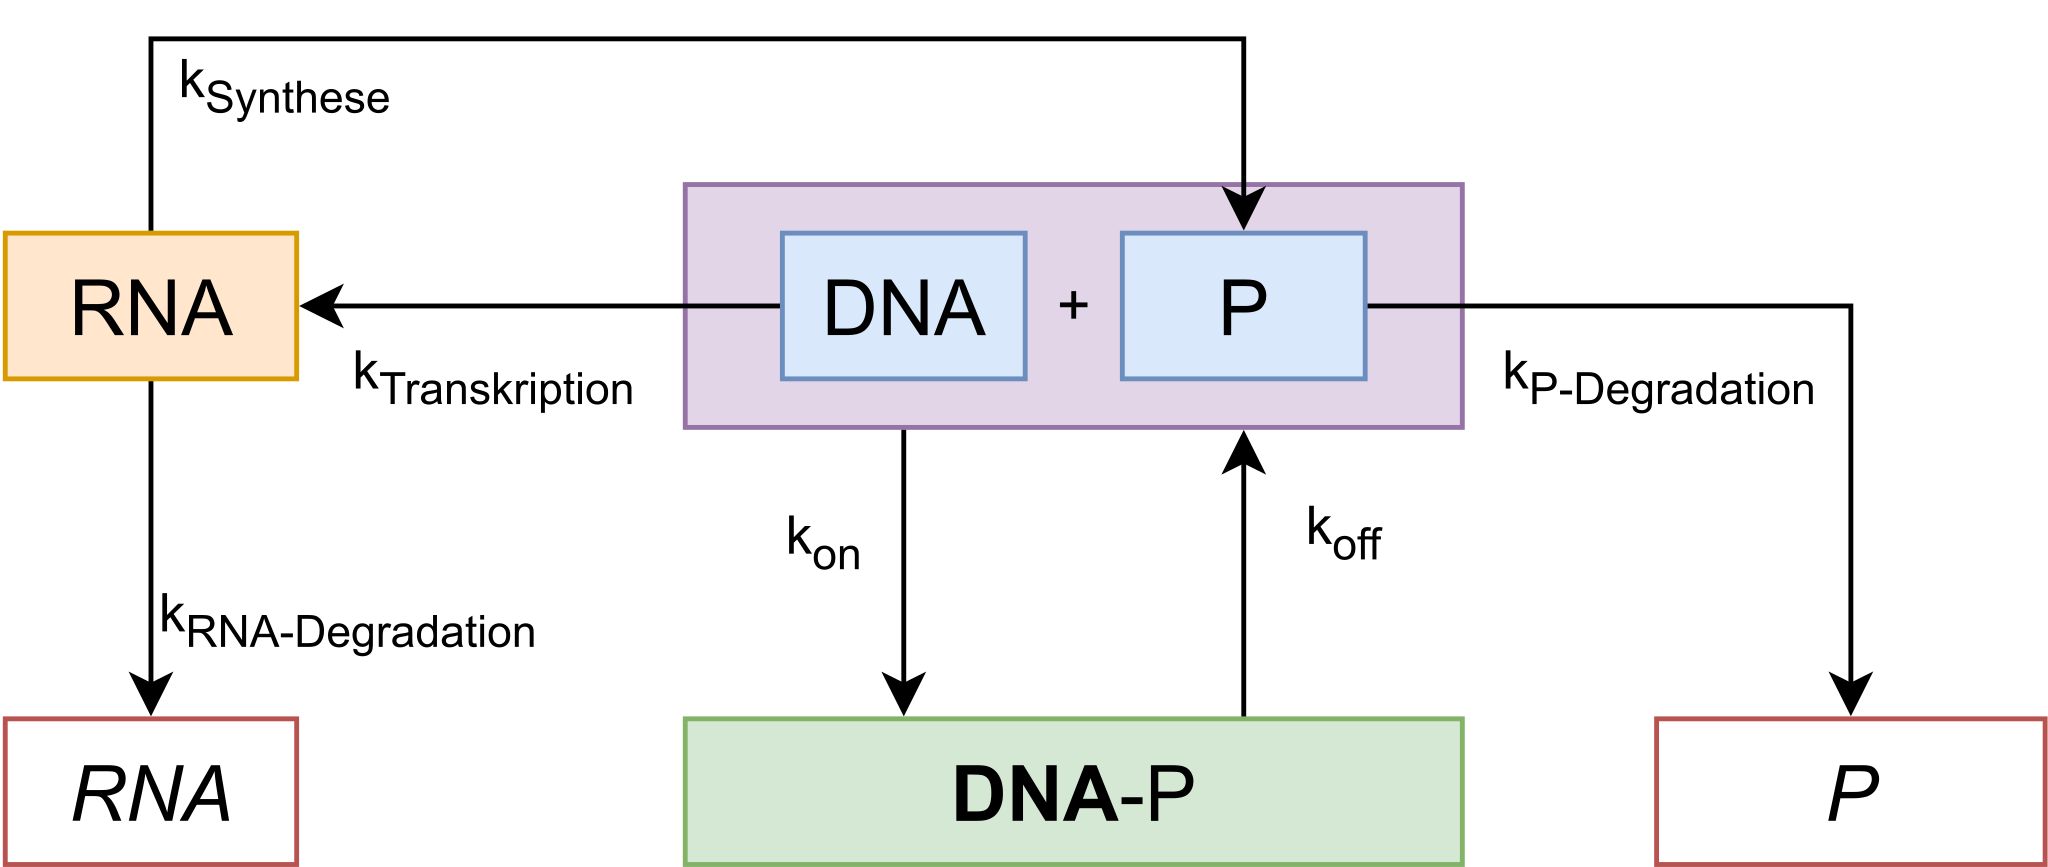
\includegraphics[width=\textwidth]{images/negative_autoregulation_overview.png}

%@Xaver
%\note{Mit Overview neuen Kontext einleiten}
\end{frame}

% Xaver
\begin{frame}{Mathematische Modellierung}
\begin{columns}
    \column{.5\textwidth}
    \includegraphics[width=\textwidth]{images/negative_autoregulation_RNA.png}
    \column{.5\textwidth}
    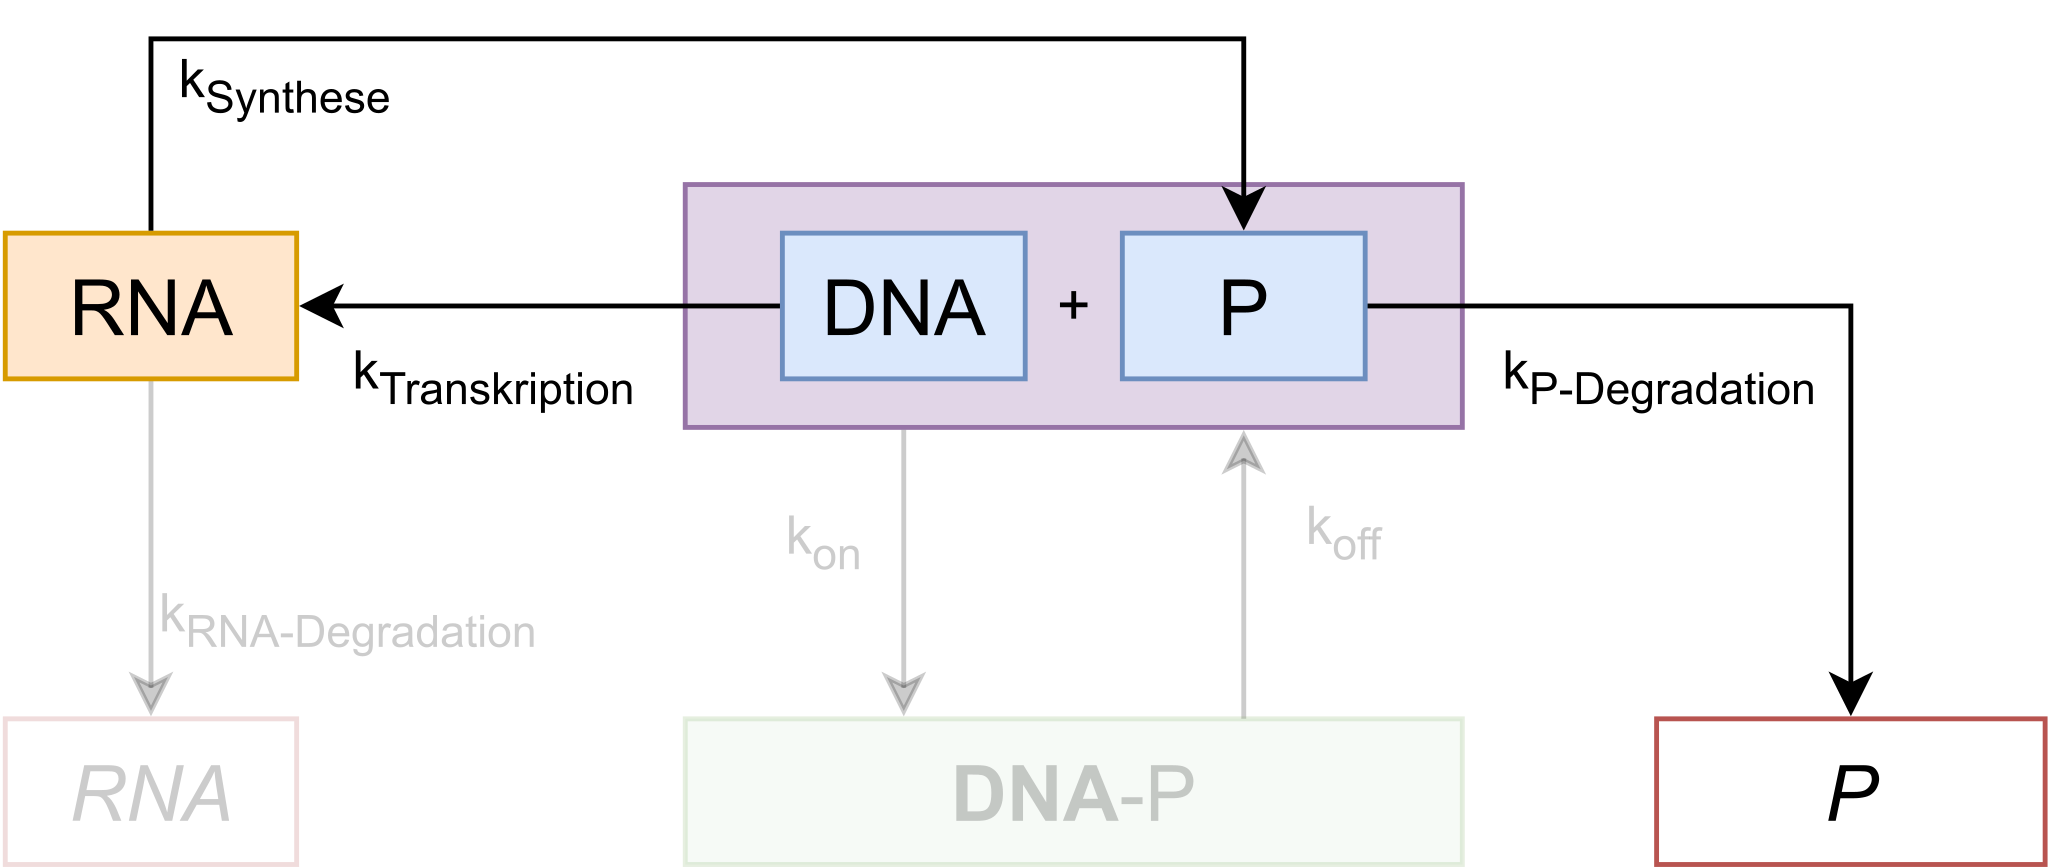
\includegraphics[width=\textwidth]{images/negative_autoregulation_P.png}
\end{columns}
\pause
\vspace{24pt}
\begin{columns}
    \column{.5\textwidth}
    \[\frac{d[\text{RNA}]}{dt}=\text{RNA}_{\text{Synthese}}-\text{RNA}_{\text{Degradation}}\]
    \column{.5\textwidth}
    \[\frac{d[\text{P}]}{dt}=\text{P}_{\text{Synthese}}-\text{P}_{\text{Degradation}}\]
\end{columns}

\end{frame}

% Xaver
\begin{frame}{Mathematische Modellierung mRNA}
    
    \begin{columns}
        \column{0.5\textwidth}
            \includegraphics[width=\textwidth]{images/negative_autoregulation_RNA.png}
        \column{0.5\textwidth}

        % pause does not work with the align environment
        \begin{align*}
            \action<+->{\frac{d[\text{RNA}]}{dt}&=\text{RNA}_{\text{Transkription}}-\text{RNA}_{\text{Degradation}}\\[2em]}
            \action<+->{\text{RNA}_{\text{Transkription}}&=}\only<+>{k_\text{t}\cdot [\text{DNA}]}\only<+->{k_{\text{t}} \cdot [\text{DNA}_\text{Total}]  \cdot \frac{K_d}{K_d+[\text{P}]}}\\
            \action<+->{\text{RNA}_{\text{Degradation}}&=}\action<+->{k_{dr} \cdot [\text{RNA}]}
        \end{align*}
    \end{columns}

    \vspace{3em}
    \[\action<+->{\frac{d[\text{RNA}]}{dt}=\action<+->{\underbrace{k_{\text{t}} \cdot [\text{DNA}_\text{Total}]}_{v_\text{max}} \cdot \frac{K_d}{K_d+[\text{P}]}-k_{dr} \cdot [\text{RNA}]}}\]
\end{frame}

% Mario
\begin{frame}{Mathematische Modellierung Protein}
    \begin{columns}
        \column{0.5\textwidth}
            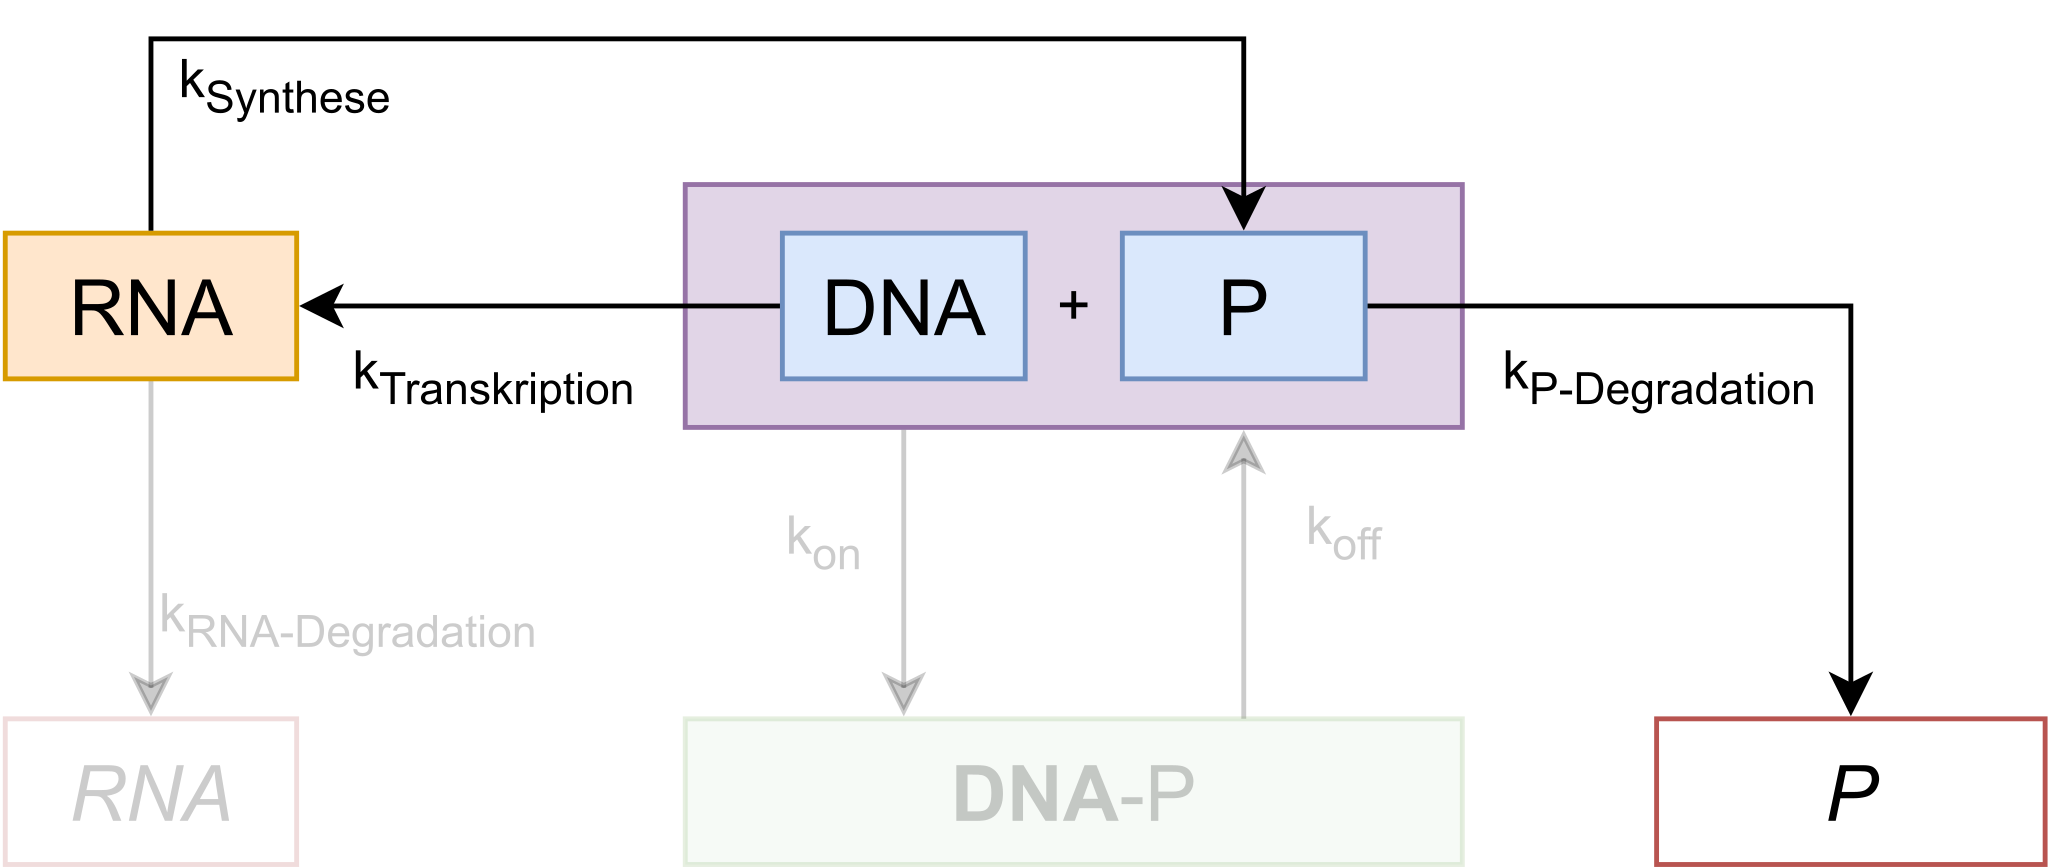
\includegraphics[width=\textwidth]{images/negative_autoregulation_P.png}
        \column{0.5\textwidth}

        \begin{align*}
            \action<+->{\frac{d[\text{P}]}{dt}&=\text{P}_{\text{Synthese}}-\text{P}_{\text{Degradation}}\\[2em]}
            \action<+->{\text{P}_{\text{Synthese}}&=\action<+->{k_s\cdot [\text{RNA}]}\\}
            \action<+->{\text{P}_{\text{Degradation}}&=\action<+->{k_{dp}\cdot [\text{P}]}}
        \end{align*}
    \end{columns}

    \vspace{3em}
    \[\action<+->{\frac{d[\text{P}]}{dt}=\action<+->{k_s\cdot[\text{RNA}]-k_{dp}\cdot[\text{P}]}}\]
\end{frame}

% Mario
\begin{frame}{Mathematische Modellierung\hfill {\small\textcolor{ETHBlue}{Negative Autoregulation}}}
    \begin{columns}
        \column{.3\textwidth}
        \includegraphics[width=\textwidth]{images/repression.png}
        \column{.7\textwidth}
        \begin{align*}
            \colorbox[HTML]{FFD966}{$\dfrac{d[\text{RNA}]}{dt}$}&=v_{\text{max}}\cdot\frac{K_d}{K_d+[\text{P}]}-k_{dr}\cdot [\text{RNA}]\\[16pt]
            \colorbox[HTML]{A680B8}{$\dfrac{d[\text{P}]}{dt}$}&=k_s\cdot[\text{RNA}]-k_{dp}\cdot[\text{P}]
        \end{align*}
    \end{columns}
\end{frame}

\begin{frame}[t]{Stationäre Lösung herleiten}
    \begin{columns}[t]
        \column{.5\textwidth}
            \[\frac{d[\text{RNA}]}{dt}=v_{\text{max}}\cdot\frac{K_d}{K_d+[\text{P}]}-[\text{RNA}] \cdot k_{dr}\]
        \column{.5\textwidth}
            \[\frac{d[\text{P}]}{dt}= k_s\cdot[\text{RNA}]-k_{dp}\cdot[\text{P}]\]
    \end{columns}
\end{frame}

% Xaver
\begin{frame}[t]{Stationäre Lösung herleiten}
    \begin{columns}[t]
        \column{.5\textwidth}
            \[0=v_{\text{max}}\cdot\frac{K_d}{K_d+[\text{P}]}-[\text{RNA}] \cdot k_{dr}\]
        \column{.5\textwidth}
            \[0= k_s\cdot[\text{RNA}]-k_{dp}\cdot[\text{P}]\]
    \end{columns}
    \pause
    \begin{columns}[t]
        \column{.5\textwidth}
            
        \column{.5\textwidth}
            \[\Rightarrow \textcolor{ETHPurple}{[\text{RNA}]}=\frac{k_{dp} \cdot [\text{P}]}{k_s}\]
    \end{columns}
    \pause
    \begin{columns}[t]
        \column{.5\textwidth}
            \[0=v_{\text{max}}\cdot\frac{K_d}{K_d+[\text{P}]}-\textcolor{ETHPurple}{[\text{RNA}]} \cdot k_{dr}\]
            \pause
            \[0=v_{\text{max}}\cdot\frac{K_d}{K_d+[\text{P}]}-\textcolor{ETHPurple}{\frac{k_{dp} \cdot [\text{P}]}{k_s}} \cdot k_{dr}\]
            \pause
            \[0=[\text{P}]^2 \cdot \underbrace{k_{dp} \cdot k_{dr}}_{a} + [\text{P}] \cdot \underbrace{K_d \cdot k_{dp} \cdot k_{dr}}_{b} - \underbrace{v_{\text{max}} \cdot K_d \cdot k_s}_{c}\]
            \pause
        \column{.5\textwidth}
    \end{columns}
    \begin{columns}[t]
        \column{.5\textwidth}
            \[\Downarrow\text{Mitternachtsformel(a,b,c)}\]
            \[[\text{P}] = \]
        \column{.5\textwidth}
        \[[\text{RNA}] = \]
    \end{columns}

\end{frame}

% Xaver
\begin{frame}{Konstanten}
    \renewcommand{\arraystretch}{2}
    \begin{tabular}{m{.4\textwidth}|p{.2\textwidth}|p{.3\textwidth}}
        \multirow{3}*{$\dfrac{d[\text{RNA}]}{dt}=v_\text{max}\cdot\dfrac{K_d}{K_d+[\text{P}]}-k_{dr}\cdot [\text{RNA}]$}
        & $v_\text{max}$ & $15\text{ nM min$^{-1}$}$ \\
        & $K_d$ & $10^{-2}\text{ nM}=10^{-11}\text{ M}$ \\
        & $k_\text{dr}$ & $0.23\text{ min$^{-1}$}$ \\
        \hline
        \multirow{2}*{$\dfrac{d[\text{P}]}{dt}=k_s\cdot[\text{RNA}]-k_{dp}\cdot[\text{P}]$}
        & $k_\text{s}$ & $20\text{ min$^{-1}$}$ \\
        & $k_\text{dp}$ & $0.011\text{ min$^{-1}$}$ \\
    \end{tabular}
\end{frame}

\begin{frame}[t]{Stationäre Lösung herleiten}
    \begin{columns}[t]
        \column{.5\textwidth}
            \[0=v_{\text{max}}\cdot\frac{K_d}{K_d+[\text{P}]}-[\text{RNA}] \cdot k_{dr}\]
        \column{.5\textwidth}
            \[0= k_s\cdot[\text{RNA}]-k_{dp}\cdot[\text{P}]\]
    \end{columns}
    
    \begin{columns}[t]
        \column{.5\textwidth}
            
        \column{.5\textwidth}
            \[\Rightarrow \textcolor{ETHPurple}{[\text{RNA}]}=\frac{k_{dp} \cdot [\text{P}]}{k_s}\]
    \end{columns}
    
    \begin{columns}[t]
        \column{.5\textwidth}
            \[0=v_{\text{max}}\cdot\frac{K_d}{K_d+[\text{P}]}-\textcolor{ETHPurple}{[\text{RNA}]} \cdot k_{dr}\]
            
            \[0=v_{\text{max}}\cdot\frac{K_d}{K_d+[\text{P}]}-\textcolor{ETHPurple}{\frac{k_{dp} \cdot [\text{P}]}{k_s}} \cdot k_{dr}\]
            
            \[0=[\text{P}]^2 \cdot \underbrace{k_{dp} \cdot k_{dr}}_{a} + [\text{P}] \cdot \underbrace{K_d \cdot k_{dp} \cdot k_{dr}}_{b} - \underbrace{v_{\text{max}} \cdot K_d \cdot k_s}_{c}\]
        \column{.5\textwidth}
    \end{columns}
    \begin{columns}[t]
        \column{.5\textwidth}
            \[\Downarrow\text{Mitternachtsformel(a,b,c)}\]
            \[[\text{P}] = \pm34.43\text{ nM}\]
        \column{.5\textwidth}
            \[[\text{RNA}] = \pause \frac{k_{dp} \cdot 34.43\text{ nM}}{k_s}\]
            \[[\text{RNA}] = 0.0189\text{ nM}\]
    \end{columns}

\end{frame}

\begin{frame}{Numerische Lösungen mit MATLAB}
    Simulation des Modells mit bestimmten Anfangswerten
    \begin{itemize}
        \item[$\Rightarrow$] keine Störungen
        \item[$\Rightarrow$] System sollte zu einem Gleichgewicht tendieren
    \end{itemize}

    \vspace{4em}
    \textbf{Was ist MATLAB?}\\
    \begin{itemize}
        \item Programmiersprache und -umgebung zum Lösen mathematischer Probleme
        \item \emph{Verfügt über mehrere Funktionen, Differentialgleichungen zu lösen}
        \item Verschiedenste Module unterschiedlicher Anwendungsfelder wie z.B. Computational Biology
    \end{itemize}
\end{frame}

% Mario
\begin{frame}{Numerische Lösung mit MATLAB\hfill {\small \textcolor{ETHBlue}{Negative Autoregulation}}}
\begin{figure}
    \centering
    \includegraphics[width=.7\textwidth]{images/simulations/negative_autoregulation_basic.m.png}
\end{figure}
\end{frame}

\begin{frame}{Numerische Lösung mit MATLAB\hfill {\small \textcolor{ETHBlue}{Negative Autoregulation}}}
    \begin{columns}
        \column{.4\textwidth}
            \textbf{Gleichgewichtszustand}\\[1em]
            
            \begin{itemize}
                \item $\text{RNA}_\text{Synthese}=\text{RNA}_\text{Degradation}$
                \item $\text{Protein}_\text{Synthese}=\text{Protein}_\text{Degradation}$
                \vspace{1em}
                \item RNA bei ungefähr 0.02 nM
                \begin{itemize}
                    \item \emph{\tiny Vorausgesagt: $0.0189\text{ nM}$}
                \end{itemize}
                \item Protein bei ungefähr 34.5 nM
                \begin{itemize}
                    \item \emph{\tiny Vorausgesagt: $34.43\text{ nM}$}
                \end{itemize}

                \item $\dfrac{[\text{RNA}]}{[\text{Protein}]}\approx \dfrac{1}{1725}$
            \end{itemize}
        \column{.6\textwidth}
        
        \begin{figure}
            \centering
            \includegraphics[width=\linewidth]{images/simulations/negative_autoregulation_basic.m.png}
        \end{figure}
    \end{columns}
\end{frame}

\begin{frame}{Unterschiedliche Bedingungen\hfill {\small \textcolor{ETHBlue}{Negative Autoregulation}}}
    \begin{columns}
        \column{.6\textwidth}
        \begin{itemize}
            \item $[\text{P}]_0=0$ eher unwahrscheinlich
            \begin{itemize}
                \item Gleichgewichtszustand wird aber trotzdem immer erreicht
                \item $[\text{P}]_0=38\text{ nM}$
                \item[$\Rightarrow$] RNA geht direkt zum GGW-Zustand, ohne Überschuss
            \end{itemize}
        \end{itemize}
        
        \column{.4\textwidth}
        \begin{figure}
            \centering
            \includegraphics[width=\linewidth]{images/simulations/negative_autoregulation_high_protein.m.png}
        \end{figure}
    \end{columns}
    \pause

    \begin{columns}
        \column{.6\textwidth}
        \begin{itemize}
            \item Affinität des Repressors zur DNA ($K_d$) hat grossen Einfluss auf die Gleichgewichtskonzentration
            \begin{itemize}
                \item $K_d=1\text{ nM}$
                \item Je kleiner die Affinität ($\uparrow K_d$), desto höher die GGW-Konzentration
            \end{itemize}
        \end{itemize}
        \column{.4\textwidth}

        \begin{figure}
            \centering
            \includegraphics[width=\linewidth]{images/simulations/negative_autoregulation_low_affinity.m.png}
        \end{figure}
    \end{columns}
\end{frame}

\begin{frame}{Unterschiedliche Bedingungen\hfill {\small \textcolor{ETHBlue}{Negative Autoregulation}}}
    \begin{columns}
        \column{.6\textwidth}
        \begin{itemize}
            \item Degradationsraten bestimmen die Zeit bis zum Gleichgewicht
            \begin{itemize}
                \item $k_{dr}=0.46\text{ min$^{-1}$}$
                \item $k_{dp}=0.22\text{ min$^{-1}$}$
                \item Je schneller die Degradation, desto eher stellt sich ein neuer GGW ein
            \end{itemize}
        \end{itemize}
        
        \column{.4\textwidth}
        \begin{figure}
            \centering
            \includegraphics[width=\linewidth]{images/simulations/negative_autoregulation_quicker_degradation.m.png}
        \end{figure}
    \end{columns}
\end{frame}

\begin{frame}[fragile]{Code\hfill {\small \textcolor{ETHBlue}{Negative Autoregulation}}}
    \begin{figure}
        \centering
        \includegraphics[height=.8\textheight]{images/code.png}
    \end{figure}
\end{frame}

\begin{frame}{Mathematische Modellierung\hfill {\small\textcolor{ETHBlue}{Positive Autoregulation}}}
    \begin{columns}
        \column{.3\textwidth}
        \includegraphics[width=\textwidth]{images/induction.png}
        \column{.7\textwidth}
        \begin{align*}
            \colorbox[HTML]{FFD966}{$\dfrac{d[\text{RNA}]}{dt}$}&=v_{\text{max}}\cdot\textcolor{ETHRed}{\frac{[\text{P}]}{K_d+[\text{P}]}}-k_{dr}\cdot [\text{RNA}]\\[16pt]
            \colorbox[HTML]{A680B8}{$\dfrac{d[\text{P}]}{dt}$}&=k_s\cdot[\text{RNA}]-k_{dp}\cdot[\text{P}]
        \end{align*}
    \end{columns}
\end{frame}

% Mario
\begin{frame}{Numerische Lösung mit MATLAB\hfill {\small\textcolor{ETHBlue}{Positive Autoregulation}}}
    \begin{columns}
        \column{.5\textwidth}
        \begin{figure}
            \centering
            \includegraphics[width=\linewidth]{images/simulations/positive_autoregulation_basic.m.png}
        \end{figure}

        \column{.6\textwidth}
        \begin{itemize}
            \item Gleiche Parameter wie für negative Autoregulation
            \begin{itemize}
                \item $[\text{P}]_0=10\text{ nM}$
                \item $[\text{P}]_0=0\text{ nM}$ würde zu keiner Expression führen
            \end{itemize}
            \item Gleichgewichtskonzentration limitiert durch $v_\text{max}$\\ {\tiny vgl. Folie 3}
            \item Gleichgewichtszustand deutlich langsamer erreicht
            \item Falls Initialkonzentration über GGW-Konzentration
            \begin{itemize}
                \item Proteinkonzentration fällt hinunter zum GGW
                \item Kaum Einfluss auf RNA-Produktion
            \end{itemize}
            \item $\dfrac{[\text{RNA}]}{[\text{Protein}]}\approx \dfrac{1}{1550}$
        \end{itemize}
    \end{columns}
\end{frame}

\begin{frame}{Biologische Verwendungen}
    \begin{columns}
        \column{.5\textwidth}
        \centering
        \textbf{Positive Autoregulation}
        \begin{figure}
            \includegraphics[width=.6\textwidth]{images/dna_positive_autoregulation.png}
        \end{figure}

        \begin{itemize}
            \item All-or-Nothing response
            \item Zwei stabile Zustände (an oder aus)
            \item Zustand ist durch Mitose vererbar
            \item Tochterzellen behalten so denselben Typ
        \end{itemize}
        
        \column{.5\textwidth}
        \centering
        \textbf{Negative Autoregulation}
        \begin{figure}
            \includegraphics[width=.6\textwidth]{images/dna_negative_autoregulation.png}
        \end{figure}

        \begin{itemize}
            \item Proteinkonzentration wird auf einem konstanten Level gehalten
            \item Abweichungen führen zu sehr schneller Antwort
            \item Korrektur erfolgt in beide Richtungen 
        \end{itemize}
    \end{columns}
\end{frame}

% TBD
\begin{frame}{Erweiterungen des Modells}
    \begin{columns}
        \column{.5\textwidth}
        \begin{itemize}
            \item Beachtung von Verzögerungen in der Transkription und Translation
            \item Verdünnung durch Zellwachstum
            \item DNA-Bindeproteine sind oft kooperativ
            \item Nacheinanderschaltung von verschiedenen "Schaltkreisen"
            \item ...
            \item Abbildung von echt vorkommenden Genen wie z.B. das Lac Operon
        \end{itemize}
        
        \column{.5\textwidth}
        \begin{figure}
            \centering
            \includegraphics[width=\textwidth]{images/network.png}
        \end{figure}
    \end{columns}
\end{frame}

\begin{frame}{Abschluss}
    \centering
    Danke an Florin Gegenschatz, Dr. Alexander Caspar und Ana Kitanovic für die Unterstützung!

    \vspace{4em}
    \emph{Wer Lust auf mehr hat}\\[1em] 
    Molecular Biology of the Cell, Chapter 8, Mathematical Analysis of Cell Functions\\[.5em]
    4. Semester, Systembiologie
\end{frame}

\end{document}